% Бүлэг 1

\chapter{Прокси дахин шифрлэлтэд суурилсан файл хуваалцах систем хөгжүүлэх}

\label{Chapter3} % Энэ бүлэг рүү ишлэл хийх бол \ref{Chapter1} командыг ашигла 
\pagecolor{white}

%-------------------------------------------------------------------------------
%	SECTION 1
%-------------------------------------------------------------------------------
\section{Системийн шаардлага}
Систем нь түлхүүр үүсгэх файл хадгалах сервер, өгөгдөл эзэмшигч, өгөгдөл хэрэглэгч гэсэн үндсэн гурван хэсгээс тогтоно. Өгөгдөл эзэмшигч бүртгэл үүсгэж өөрийн нийтийн түлхүүр болон хувийн түлхүүрийг үүсгэж авна. Файл шифрлэх болон тайлах үйлдлийг өөрийн төхөөрөмж дээр үйлдэнэ.

\textbf{Системийн оролцогч}
\begin{itemize}
    \item Хэрэглэгч
\end{itemize}

\textbf{Системийн тоглогч}
\begin{itemize}
    \item Файл эзэмшигч
    \item Файл хэрэглэгч
\end{itemize}

\subsection*{Функцийн шаардлага}
Файл эзэмшигчийн функционал шаардлага:
\begin{itemize}
    \item Системд өөрийн бүртгэлийг үүсгэх
    \item Файл оруулах, шифрлэх
    \item Файлыг тайлах хэрлэгч сонгох
    \item Шифрлэсэн файлыг хуваалцсан хэрлэгчдийн жагсаалт
\end{itemize}
Файл хэрэглэгчийн функционал шаардлага:
\begin{itemize}
    \item Системд өөрийн бүртгэлийг үүсгэх
    \item Өөрт хуваацлсан файлын жагсаалт
    \item Файлыг татаж авах
    \item Шифрлэсэн файлыг тайлах
\end{itemize}

\subsection*{Функцийн бус шаардлага}
\begin{enumerate}
    \item Файлыг шифрлэх, шифрийг тайлах хурдан гүйцэтгэдэг байх
    \item Хэрэглэгчийн интерфейс ойлгомжтой энгийн байх.
    \item Прокси серверт файлыг шифрлэсэн байдлаар хадгалах, хуваалцах
    \item Өөрийн бүртгэлийг ашиглаж нэвтрэх
    \item Хувийн түлхүүрийг хэрлэгчийн төхөөрөмж дээр авч явах
\end{enumerate}

\subsection*{Юзкейс диаграмм}
Системийн хэрлэгчид ямар үйлдлүүдийг системд хийж болохыг харуулсан хэрэглээний диаграммыг харууллаа.
\begin{figure}[ht]
    \centering
    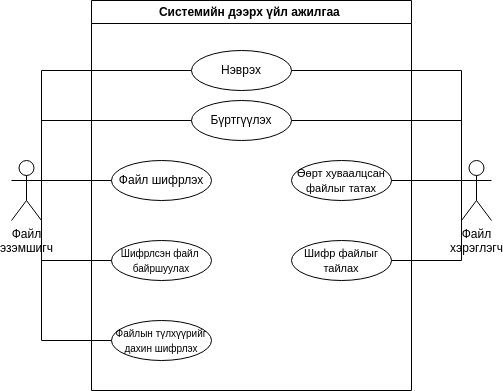
\includegraphics[scale=0.6]{Figures/usecase.drawio.png}
    \caption[Usecase diagram]{Юзкейс диаграмм}
    \label{fig:usecase}
\end{figure}
\subsection*{Юзкейс тодорхойлолт}

\begin{table}
    \label{tab:treatments}
    \footnotesize
    \centering
    \begin{tabularx}{\textwidth}{|>{\hsize=0.3\hsize}X|>{\hsize=0.7\hsize}X|}
        \hline
        \multicolumn{2}{|c|}{Бүртгүүлэх} \\
        \hline
        ID & 1 \\
        \hline
        Үндсэн тоглогч & Файл эзэмшигч болон файл хэрэглэгч\\
        \hline
        Тодорхойлолт & Хэрэглэгч шинээр бүртгэл үүсгэх\\
        \hline
        Өмнөх нөхцөл & Шинэ хэрлэгч байх\\
        \hline
        Үндсэн урсгал & Хэрэглэгчийн мэдээллийг авч өгөгдлийн санд шинэ хэрэглэгч үүсгэх\\
        \hline
        Дараах нөхцөл & Хэрэглэгч өөрийн бүртгэлтэй болох нэвтрэх боломжтой болох\\
        \hline
    \end{tabularx}
    \caption{Бүртгүүлэх юзкейсийн тодорхойлолт}
\end{table}

\begin{table}
    \label{tab:treatments}
    \footnotesize
    \centering
    \begin{tabularx}{\textwidth}{|>{\hsize=0.3\hsize}X|>{\hsize=0.7\hsize}X|}
        \hline
        \multicolumn{2}{|c|}{Нэвтрэх} \\
        \hline
        ID & 2\\
        \hline
        Үндсэн тоглогч & Файл эзэмшигч болон файл хэрэглэгч\\
        \hline
        Тодорхойлолт & Системд нэвтрэх\\
        \hline
        Өмнөх нөхцөл & Бүргэлтэй хэрлэгч байх\\
        \hline
        Үндсэн урсгал & Хэрлэгчийн нууц үг бүртгэл таарч байгааг шалган нэвтрүүлэх\\
        \hline
        Дараах нөхцөл & Бусад хэрэглээ рүү хандах боломжтой болох\\
        \hline
    \end{tabularx}
    \caption{Нэвтрэх юзкейсийн тодорхойлолт}
\end{table}

\begin{table}
    \label{tab:treatments}
    \footnotesize
    \centering
    \begin{tabularx}{\textwidth}{|>{\hsize=0.3\hsize}X|>{\hsize=0.7\hsize}X|}
        \hline
        \multicolumn{2}{|c|}{Файл шифрлэх} \\
        \hline
        ID & 3 \\
        \hline
        Үндсэн тоглогч & Файл эзэмшигч\\
        \hline
        Тодорхойлолт & Файл эзэмшигч файлыг шифрлэх\\
        \hline
        Өмнөх нөхцөл & Систем нэвтэрсэн байх\\
        \hline
        Үндсэн урсгал &
            \item Файлыг сонгох
            \item Санамсаргүй байдлаар түлхүүр үүсгэх
            \item Файлыг тухайн түлхүүрээр шифрлэх
        \\
        \hline
        Дараах нөхцөл & Тухайн төхөөрөмж дээр шифрлэгдсэн байх\\
        \hline
    \end{tabularx}
    \caption{Файл шифрлэх юзкейсийн тодорхойлолт}
\end{table}

\begin{table}
    \label{tab:treatments}
    \footnotesize
    \centering
    \begin{tabularx}{\textwidth}{|>{\hsize=0.3\hsize}X|>{\hsize=0.7\hsize}X|}
        \hline
        \multicolumn{2}{|c|}{Шифрлэсэн файл серверт байршуулах} \\
        \hline
        ID & 4 \\
        \hline
        Үндсэн тоглогч & Файл эзэмшигч\\
        \hline
        Тодорхойлолт & Шифрлэсэн файлыг серверт хуулна\\
        \hline
        Өмнөх нөхцөл & Файлыг шифрэлсэн байх\\
        \hline
        Үндсэн урсгал &
            \item Шифрлэсэн файлыг серверт илгээж
            \item Файлын мэдээллийг өгөгдлийн санд нэмэх 
        \\
        \hline
        Дараах нөхцөл & Файлын талаар мэдээллийг авах боломжтой болох\\
        \hline
    \end{tabularx}
    \caption{Шифрлэсэн файл серверт байршуулах юзкейсийн тодорхойлолт}
\end{table}

\begin{table}
    \label{tab:treatments}
    \footnotesize
    \centering
    \begin{tabularx}{\textwidth}{|>{\hsize=0.3\hsize}X|>{\hsize=0.7\hsize}X|}
        \hline
        \multicolumn{2}{|c|}{Файл хуваалцах} \\
        \hline
        ID & 5 \\
        \hline
        Үндсэн тоглогч & Файл эзэмшигч\\
        \hline
        Тодорхойлолт & Файл эзэмшигч файл хуваалцах хүнийг сонгох\\
        \hline
        Өмнөх нөхцөл & Файлыг серверт байршуулсан байх\\
        \hline
        Үндсэн урсгал &
            \item Файл хуваалцах хүний нийтийн түлхүүрийг авах
            \item Дахин шифрлэх түлхүүр үүсгэх
            \item Файлыг дахин шифрлэх\\
        \hline
        Дараах нөхцөл & Шифрлэсэн файлыг төхөөрөмж дээр тайлхда бэлэн болох\\
        \hline
    \end{tabularx}
    \caption{Файл хуваалцах юзкейсийн тодорхойлолт}
\end{table}

\begin{table}
    \label{tab:treatments}
    \footnotesize
    \centering
    \begin{tabularx}{\textwidth}{|>{\hsize=0.3\hsize}X|>{\hsize=0.7\hsize}X|}
        \hline
        \multicolumn{2}{|c|}{Файл татах} \\
        \hline
        ID & 6 \\
        \hline
        Үндсэн тоглогч & Файл хэрэглэгч\\
        \hline
        Тодорхойлолт & Дахин шифрлэсэн файлыг татаж авах\\
        \hline
        Өмнөх нөхцөл & Файлыг хуваалцсан байх\\
        \hline
        Үндсэн урсгал & Файлыг татаж авах\\
        \hline
        Дараах нөхцөл & Файлыг тайлхад бэлэн болох\\
        \hline
    \end{tabularx}
    \caption{Файл татах юзкейсийн тодорхойлолт}
\end{table}

\begin{table}
    \label{tab:treatments}
    \footnotesize
    \centering
    \begin{tabularx}{\textwidth}{|>{\hsize=0.3\hsize}X|>{\hsize=0.7\hsize}X|}
        \hline
        \multicolumn{2}{|c|}{Шифрлэсэн файлын тайлах} \\
        \hline
        ID & 7 \\
        \hline
        Үндсэн тоглогч & Файл хэрэглэгч\\
        \hline
        Тодорхойлолт & Татаж авсан шифрлэсэн файлыг тайлах\\
        \hline
        Өмнөх нөхцөл & Файлыг хуваалцсан байх\\
        \hline
        Үндсэн урсгал & 
        \item Файлын түлхүүрийг өөрийн хувийн түлхүүрээр тайлах
        \item Файлын түлхүүрээр файлыг тайлах\\
        \hline
        Дараах нөхцөл & Файлыг унших боломжтой болгох\\
        \hline
    \end{tabularx}
    \caption{Шифрлэсэн файлын тайлах юзкейсийн тодорхойлолт}
\end{table}

%-------------------------------------------------------------------------------
%	SECTION 2
%-------------------------------------------------------------------------------
% \section{Системийн загвар}

% \subsection*{Үйл ажилгааны диаграмм}

% \subsection*{Өгөгдлийн сангийн бүтэц}

%-------------------------------------------------------------------------------
%	SECTION 3
%-------------------------------------------------------------------------------
% \section{Системийн хөгжүүлэх}

%-------------------------------------------------------------------------------
%	SECTION 4
%-------------------------------------------------------------------------------
% \section{Файл хуваалцах системийг турших}

%-------------------------------------------------------------------------------
%	SECTION 5
%-------------------------------------------------------------------------------

% \section{Дүгнэлт}

